\chapter{引言}
% 解释:RISC-V、开源处理器、高性能、虚拟化、虚拟化扩展
% 提及:云和数据中心领域是热的,在工业界有人不断尝试,是值得做的。
% 尽管该项目可能无法实现、但是需要去尝试、合并到工业界中。
% 以未来为切入点,画大饼。
% 历史片段

% 2018年11月8日,在网信办、中科院等多个国家部委支持和指导下,
% RISC-V中国联盟于浙江乌镇举行的第五届互联网大会上正式宣布成立。
% 从成立到现在的5年见,可以看见国内RISC-V相关产业在快速的发展。
% RISC-V是一个基于精简指令集原则的指令集架构,与x86、ARM架构是对应的关系。
% 首先,RISC-V与其他指令集最大的不同点在与开源性,即不需要收取高额的版权费,
% 相对的,x86和ARM指令集知识产权的公司均为国外公司,不利于我国实现关键芯片的自主可控。
% 因此,开源意味着自由、安全及可控。
% 其次,RISC-V还具有简洁、模块化的特点,
% 意味着轻量化、低功耗、小体积,因此非常适用于移动设备,以及在多场景的灵活适应性。
% 正是具有以上特点,在计算机体系结构领域,RISC-V受到了学术界和工业界的广泛瞩目。
% 短短六年,中国目前有300家以上公司在关注RISC-V或以RISC-V指令集进行开发。
% 从嵌入式到AI服务器,各种类别的RISC-V处理器核百花齐放。
% 我们有理由相信,未来RISC-V将在中国的芯片领域有更大的应用空间和市场份额。

% 中科院计算所研究员孙凝晖院士如此说道:“
% 开源模式不仅仅是一种商业模式,也是一种生态构建方法,是一种复杂系统开发方法。
% 更蕴含着一种精神。开源不仅仅公开源代码,更重要的是协作开发流程的建立与社区治理机制的建设。”

% 和中国知网上收录的关于RISC-V的文章在2018到2023年的平均增长比例达到了17.21\%和17.37\%

% RISC-V重要性,RISC-V是什么
% 虚拟化技术的重要性,什么是虚拟化技术
% RISC-V也在不断迈向虚拟化技术,这是十分必要的一件事
% 最后说出我们的工作内容,在这里不用说调试的问题


虚拟化技术,作为计算机科学领域的一项关键技术,为云数据中心提供的各类服务构建了核心的技术框架。
通过在计算机硬件上创建一个抽象层,虚拟化技术能够将单台计算机的硬件分成多个虚拟计算机。
每个虚拟机能够运行自己的操作系统,和其他虚拟机相互独立,同时又能被简单且可复现地构建、销毁。
这些优势与云计算的发展方向和对灵活IT解决方案的需求十分契合,真正改变了过去的传统物理机的数据中新模式。
随着服务器虚拟化已成为一种常见做法,许多企业已从物理现场数据中心转向虚拟化数据中心解决方案。
对于运营商而言,它能减少管理开支、减少停机时间并增强灾难恢复情况下的弹性、更加充分利用硬件资源以提高效率和生产力。
对于用户而言,能够在需要时仅购买所需的计算资源,并随着工作负载的增长经济实惠地扩展这些资源。
随着近年来云数据中心及云服务提供商的快速发展,从初期的虚拟机与容器技术,
到新兴的函数即服务(Function as a Service, FaaS)与无服务器计算(Serverless)模式,
均展现出了强烈的市场需求和广阔的发展潜力。
这一趋势不断促进虚拟化技术的进步与创新,
处理器芯片行业的主要参与者开始在主流计算架构中引入硬件虚拟化支持以加速虚拟化软件的运行,
例如,Intel VT\cite{intel-VT2005Computer}以及ARM的VE扩展\cite{armve2018}。

\begin{figure}[htbp]
\centering
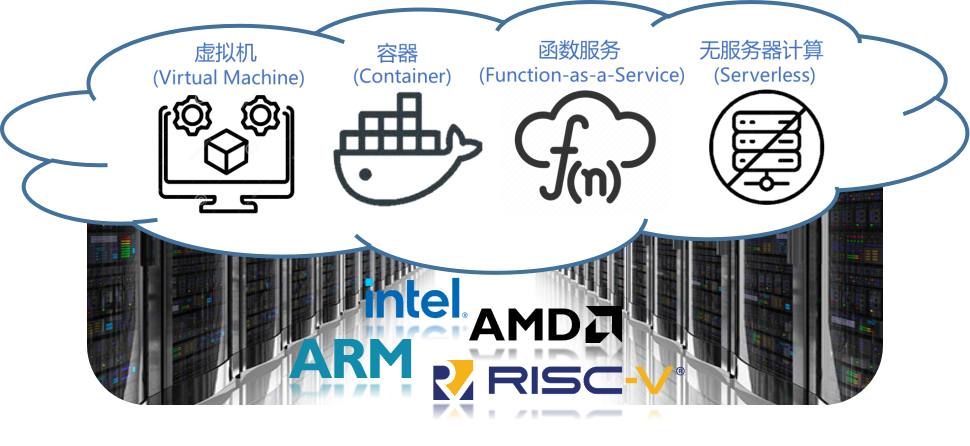
\includegraphics[scale=0.5]{virtual.png}
\caption{云数据中心在不同指令集架构的发展}
\end{figure}

然而,近年来在计算机体系结构的研究催生了一种名为RISC-V\cite{asanovic2014instruction}
的新型指令集架构(Instruction Set Architecture,ISA)。
RISC-V凭借其开源、简洁、模块化的特性,逐渐进入由x86、ARM垄断的芯片市场,也开始着手云数据中心的需求。
首先,RISC-V与其他指令集最大的不同点在与开源性,即不需要收取高额的版权费,
相对的,x86和ARM指令集知识产权的公司均为国外公司,不利于我国实现关键芯片的自主可控。
因此,开源意味着自由、安全及可控。同时,RISC-V还具有简洁、模块化的特点,
这意味着轻量化、低功耗、小体积,因此非常适用于移动设备,以及在多场景的灵活适应性。
正是具有以上特点,在计算机体系结构领域,RISC-V受到了学术界和工业界的广泛瞩目。
短短六年,中国目前有300家以上公司在关注RISC-V或以RISC-V指令集进行开发。
从嵌入式到AI服务器,各种类别的RISC-V处理器核百花齐放。

关于RISC-V虚拟化的研究尚处于起步阶段,研究潜力巨大。
2017年,RISC-V官方提出了虚拟化扩展的概念,规定了支持虚拟化的处理器需要额外添加的特权级和指令等。
截至2021年12月,虚拟化扩展才被正式批准。
同一年,加州大学的伯克利分校迈出了虚拟化扩展硬件实现的第一步。
他们研发了Rocket Chip\cite{itco2022rocket},一个开源的RISC-V顺序流水线处理器。
并在其上实现了完整的虚拟化扩展,进行了一系列虚拟化相关的评测。
但是,在真实应用场景下,处理器的情况会更为复杂,
多核乱序的高性能处理器才是虚拟化服务器的主流。
因此,本项目计划瞄准高性能RISC-V处理器的虚拟化扩展实现,开展从硬件扩展到软件适配的全系统评测的研究。

高性能RISC-V处理器的一个典型代表便是中国科学院计算技术研究所牵头发起的“香山”项目。
作为目前国际上性能最高的开源高性能RISC-V处理器核的同时,
“香山”致力成为一个开源的工业级别处理器,并成为面向世界的体系结构创新开源平台。
中科院计算所研究员孙凝晖院士对开源精神表示:“
开源模式不仅仅是一种商业模式,也是一种生态构建方法,是一种复杂系统开发方法。
更蕴含着一种精神。开源不仅仅公开源代码,更重要的是协作开发流程的建立与社区治理机制的建设。”
“香山”始终坚持、坚定地开源所有的设计、验证、基础工具代码,十分欢迎来自社区的贡献。
因此,十分适合用于高性能RISC-V处理器的虚拟化扩展研究。

本项目的尝试研究如图\ref{fig:level}虚拟化系统。
首先,在底层的硬件,需要在“香山”处理器的“南湖”架构——一个用于学术研究的稳定版本,添加虚拟化扩展。
第二,在扩展的处理器中运行虚拟机管理系统。
本项目选用经典的Type2管理系统Linux-KVM\cite{kvm:H-ext},并尝试在此基础上启动虚拟机。
最后,尝试在整个软硬件系统中,使用FPGA加速仿真平台进行系统级的评估。
然而,在启动虚拟机的过程中,由于软件复杂性和硬件处理器潜在的问题,出现了一些难以调试的错误。
此时距离处理器开始运行已经经过了很长的时钟周期,常规的调试手段难以追踪错误来源。
急需一种能够快速定位错误现场,并能够提供体系结构信息的调试工具。
为此,本项目还对处理器的调试工具进行了探索,分别在软件逻辑仿真和FPGA硬件加速仿真的两个方向上进行了尝试。

\begin{figure}[htbp]
    \centering
    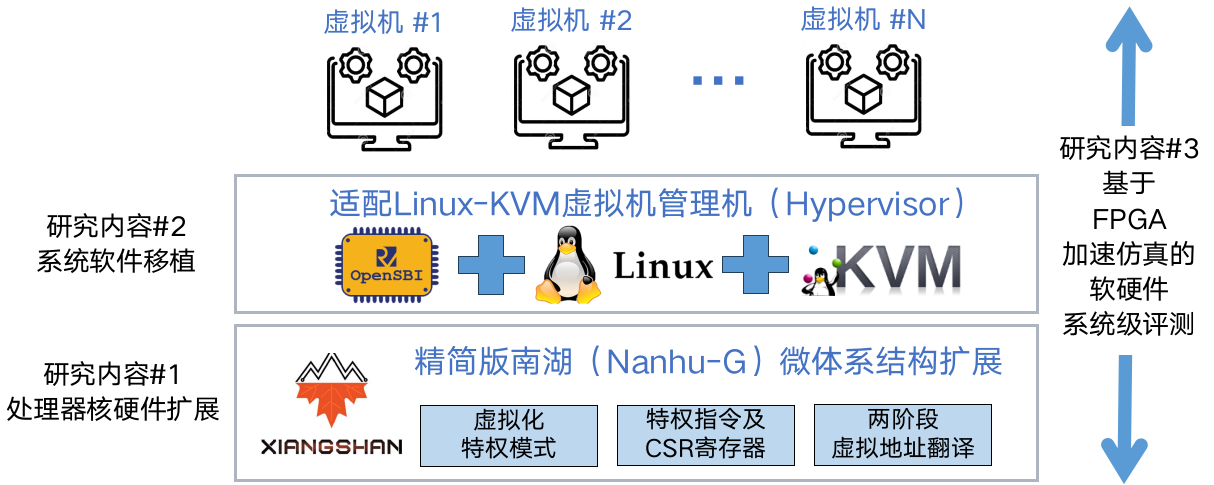
\includegraphics[scale=0.45]{level.png}
\caption{虚拟化体系结构与本项目研究内容}
    \label{fig:level}
\end{figure}
